\chapter{Objects of Research}
	This chapter defines the objects or events which will be researched in this thesis. This includes a literature review and descriptive definition of a congestion. For the use in the data analysis jam events with be further defined based on FCD.  

\section{Incident}
		Incidents in the scope of this thesis, an incident can be accidents, as well as ongoing roadwork or maintenance on the Bavarian street network. These are also the events, which the concept of the thesis tries to predict through the analysis of the correlation of said incidents to jams.
	\subsubsection{Accident}
		An accident is an unexpected and unintentional traffic event, that typically results in damages, injuries and reduction of traffic volumes. These events can be triggered by a number of different reasons, where in this thesis the main focus is on the triggers of slow, congested traffic or roadworks.
	\subsubsection{Roadwork}
		As roadwork classifies all static and moving construction sites, as well as temporary blockages or disturbance due to snow clearing, road maintenance and alike. 
	
\section{Congestion}
\label{definition_congestion}

\paragraph{Naming} As there doesn’t exist a clear plural of the noun congestion the term jams will be used in case of multiple congestion. These two terms are seen as interchangeable for their reference to a single or multiple congestion events.

\subsection{Descriptive Definition}
Jams or a single congestion in layman terms are spatial and timely accumulations of traffic participants, resulting in speeds slower or sometimes much slower than free flow. In severe cases this is also often described as stop-and-go or stopped traffic. They are triggered by a reduction of traffic throughput in volume or an increase of traffic demand. Studies have shown that these triggers are usually caused by four categories of disturbances. \parencite{TRB2003,FHA2011}

\subsubsection{Traffic-Influencing Events}

\begin{itemize}
	\item Incidents : Events that disrupt the normal free flow of traffic, like vehicular crashes, breakdowns or debris. These physical obstacles block lanes or hard shoulders, forcing other road users to execute evasive maneuver and deviate from their normal path. This ultimately changes driving behavior, reduces the quality of traffic flow and traveling speed. Even when incidents are not directly on the roadway they can impact the traffic flow due to emergency responses create blockades or ineffective driving behavior of traffic participants gapping on the incident.
	\item Roadwork : Managed and unmanaged construction sites on the roadway that result in physical changes to the highway environment. This includes a reduction of lanes, lane diversion, elimination of hard shoulders or road closures, which reduce the road capacity and reduce travel speeds.
	\item Weather : Changes in environmental conditions like heavy rain or snow fall can negatively impact driver behavior. The reduction of visibility will usually result in a reduction of traveling speeds and increase of headway. This reduces the overall capacity of the highway. Bright sunlight, smoke or icy road surfaces lead to a similar effect.
\end{itemize}

\subsubsection{Traffic Demand}

\begin{itemize}
	\item Fluctuations in Normal Traffic : Variations in demand in day-to-day traffic volumes can overload systems with fixed capacities. This can result in travel speed reductions without any specifically occurring events.
	\item Special Events : Special cases where events drastically change the demand in their vicinity and overload the system. As with incidents, off-road events can affect driving behavior due to visual distractions and change the traffic-flow. 
\end{itemize}

\subsubsection{Physical Highway Features}

\begin{itemize}
	\item Traffic Control Devices : Poorly time or defective traffic signals as well as ineffectively controlling the traffic flow contribute to the creation of jams and travel time reductions.
	\item Physical Bottlenecks or Capacity : The capacity of a road is mostly dependent on the number of lanes and hard shoulder, as well as the alignment (curves and grades). Physical changes on the road environment like in merging areas, tool booths or road endings reduce the capacity and therefore promote the formation of jams. The road capacity can also be influenced by the driving behavior, which heavily depend on the familiarity of the roadway to the driver. Drivers familiar with routinely congested tend to reduce their headway and therefore increase the capacity \parencite{Charlton2013}.
\end{itemize}

\subsubsection{Driving-behavior}
As above-mentioned, driving behavior can influence the traffic flow as well as capacity and is mostly influenced by environment and the familiarity of the road. Research showed that driving on familiar road has a negative effect on safety aspects of driving behaviors, like in-attentional blindness for roadside features \parencite{Charlton2013}. Another decreasing factor is the state-of-mind, better known as rage- or aggressive driving, resulting in rapid lane changing, cross cutting or passing on shoulders \parencite{Shinar2004}. This can lead to driving behaviors where drivers don't keep up smooth accelerations, but rather break suddenly or accelerate in rapidly, other vehicles need to react accordingly. This creates a chain reaction leading to reduced travel speed. These are called \textit{phantom jams} because they do not have any specific origin and are common in high density traffic regions like cities and high demand highways. \parencite{ASTRA2020} 

\bigskip

This general layman's definition of jams is essential correct, but not sufficient for the data scientific approach in this thesis. The Bavarian ministry for streets does not have an official definition at the time of writing and there is no unified definition or thresholds when reduced speed or time delays can classify data as a congested or slow. This makes it necessary to form a specific definition of \glspl{jam} and their speed/space/time thresholds, for the scope of this thesis. For instance the \acrshort{adac} classifies highway traffic moving with mean speed lower than 20 km/h as jammed \parencite{ADAC2019}. In Switzerland the ministry for streets has a more severe definition with a mean speed of under 10 km/h \parencite{ASTRA2020}. A definition just this available literature does not consider the data is would be applied on. Therefore the representation of the speeds occurring in jams from the FCD dataset, introduced in \cref{dataset_fcd}, should be adducted to further tailor a definition to our needs. 

\subsection{Data Scientific Definition}

\begin{figure}[ht]
	\centering
	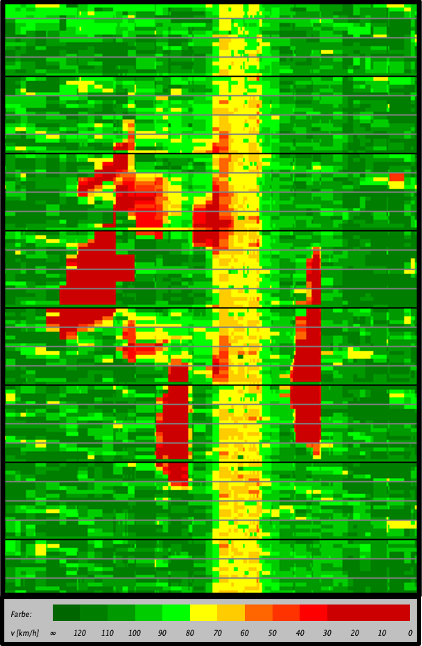
\includegraphics[scale=0.8]{images/SpeedMatrixPlot_single}
	\caption{Speed matrix plots of FCD data, showing a scattered cluster}
	\label{img:speedMatrixPlot_singleCluster}
\end{figure}

\todo{Matrix neu machen, mit bessere Lesbarkeit}

Figure \ref{img:speedMatrixPlot_singleCluster} shows a section of a random speed matrix plot from the FCD dataset, containing a scattered congestion cluster. The horizontal and vertical extend represents the spatial and temporal location of each cell. The color of the cell indicated the mean absolute speed recorded in the time frame and on the link of the cell (detailed gradient is shown in the legend of \cref{img:speedMatrixPlot_singleCluster}).

The visual representation shows that a congestion mostly contains speed of less than 30 km/h, shown in \textit{dark red}. A closer look on the cluster in the top left reveals that speed around 40-50 km/h, shown in \textit{lighter red} tones, may be also considered, to incorporate the complete congestion area. Speeds above at least 50 km/h, starting with the \textit{orange/yellow} categories, should not be included in the definition, because it would classify regular speed limits, represented by the broad vertical \textit{orange/yellow} stripe, as jammed traffic. This makes two speed threshold for jammed and slow-moving traffic necessary adequately detecting congestion clusters. With this information and some learning during calibration of the clustering algorithm (see \cref{methodology_detection_clustering}) the following thresholds for the jammed and slow speed, classifying \glspl{jam} in FCD data where defined.

\begin{itemize}
	\item Speed threshold for jammed state : $v_{crit,jammed} = 30\,\frac{km}{h}$
	\item Speed threshold for slow-moving state : $v_{crit,slow} = 60\,\frac{km}{h}$
\end{itemize}

To exclude cell errors and discard detections, too small to have to be considered as jams, the length and duration is used for filtering. 

\begin{itemize}
	\item Minimum length of a congestion : $l_{min} = 1000\,m$
	\item Minimum duration of a congestion : $t_{min} = 9\,min$
\end{itemize}

If $l < l_{min}$ or $t < t_{min}$ is given, $l$ being the maximum spatial extend and $t$ being the maximum temporal extend, the detection should be ignored.
